\begin{landscape}
\begin{figure}[H]
\centering
\caption{Circuit Scorecard (Orally Argued \& Decided Cases -- No Consolidations)}
\vspace{2.5mm}
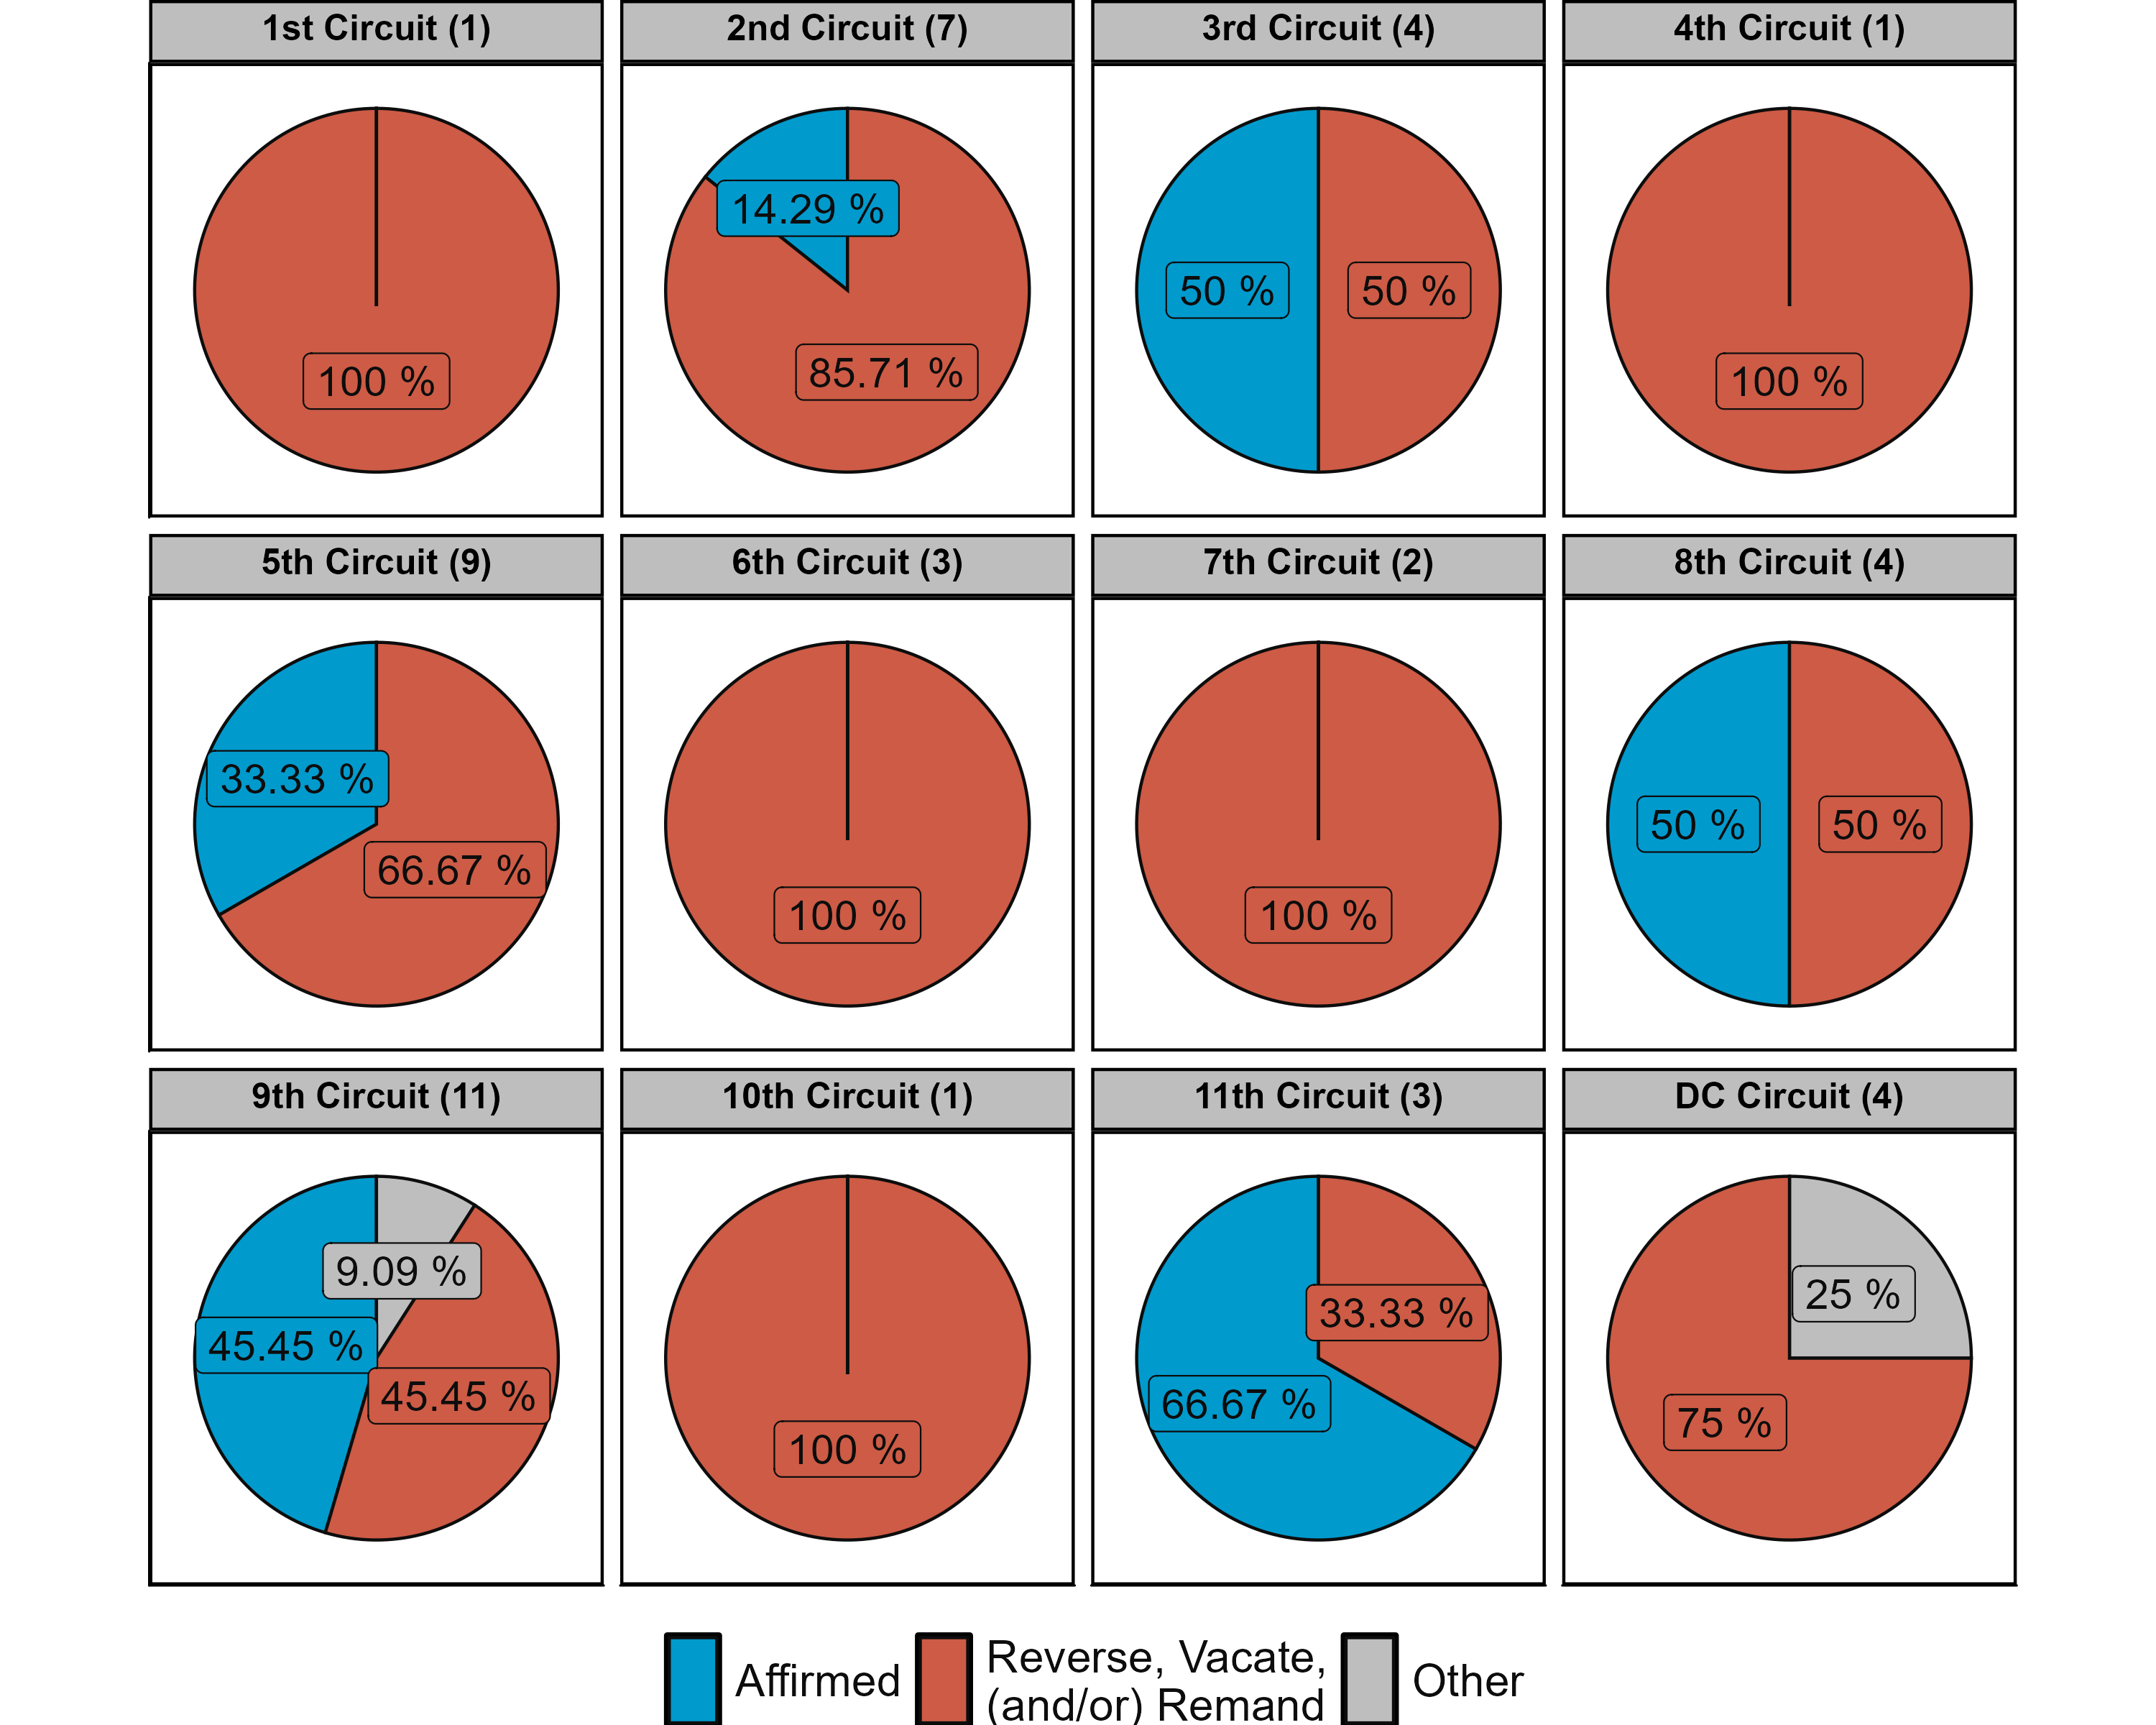
\includegraphics[width = 0.85\textwidth]{Figures/statpack_figures/circuit_scorecard_argued_decided_only.png} \\
\vspace{2.5mm}
\footnotesize{\emph{Note}: Figure considers percentage of outcomes for cases originating in respective Circuit. These only include cases that were orally argued and decided -- They do \textbf{not} consider cases that were consolidated for arguments (Ex: \emph{Danco Laboratories v. Alliance for Hipp. Medicine} with \emph{FDA v. Alliance for Hipp. Medicine}) or in rendering a decision (Ex: \emph{Relentless, Inc. v. DOC} with \emph{Loper Bright Enterprises v. Raimondo}). For percentages including those cases as well, see next page.} \\
\end{figure}
\end{landscape}

\begin{landscape}
\begin{figure}[H]
\centering
\caption{Circuit Scorecard (With Consolidations)}
\vspace{2.5mm}
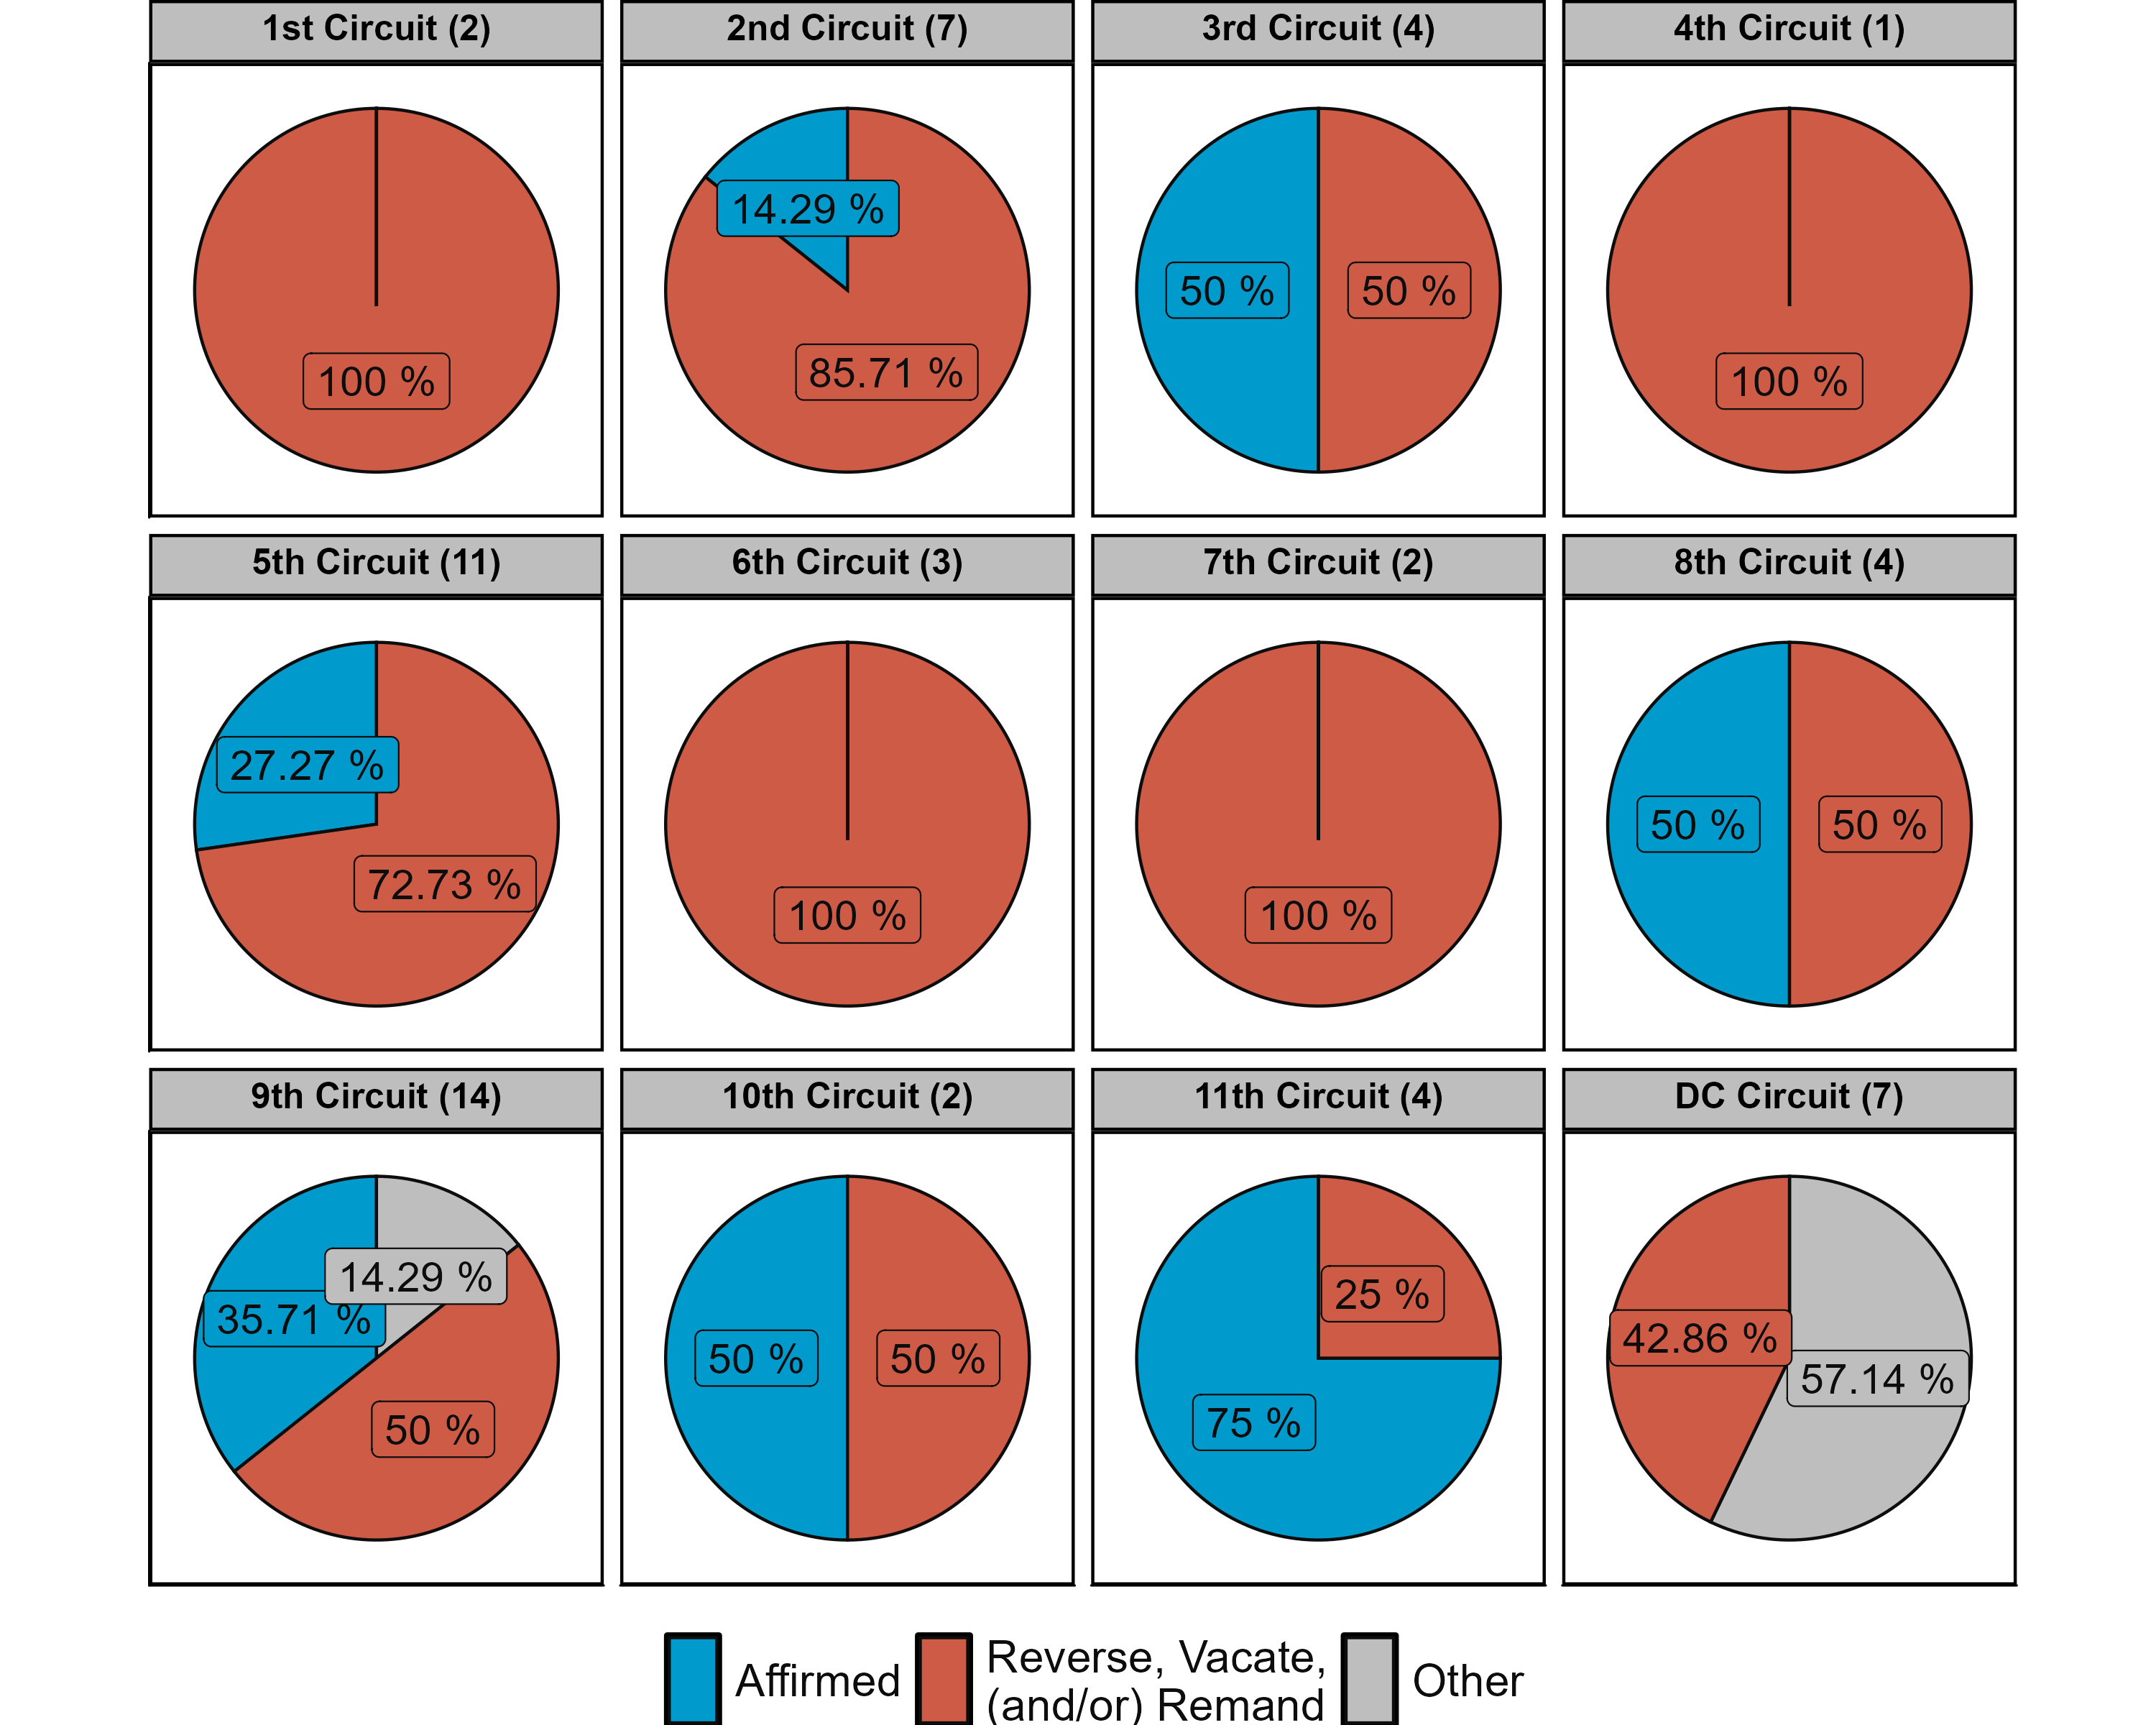
\includegraphics[width = 0.85\textwidth]{Figures/statpack_figures/circuit_scorecard_with_consolidations .png} \\
\vspace{2.5mm}
\footnotesize{\emph{Note}: This figure adds the following consolidated cases (at argument or decision level): \emph{Jackson v. U.S.} (CA11), \emph{Idaho v. U.S.} (CA9), \emph{Kinder Morgan v. EPA} (CADC), \emph{American Forest \& Paper Assn. v. EPA} (CADC), \emph{U.S. Steel Corp. v. EPA} (CADC), \emph{Becerra v. Northern Arapaho Tribe} (CA10), \emph{Danco Laboratories v. Alliance for Hipp. Medicine} (CA5), \emph{Garland v. Singh} (CA9), \emph{Garland v. Mendez Collins} (CA9), \emph{Net Choice, LLC. v. Paxton} (CA5), and \emph{Relentless, Inc. v. DOC} (CA1).}
\end{figure}
\end{landscape}
